\section{Tensegrity domes}
We will now consider the situation with added bars, but still using the constraint of fixed nodes. Our new optimisation problem has the following objective function:
\begin{equation}
\begin{aligned}
    \label{energy}
    &E(X) = \sumset{B}\big(\ebe + \ebg\big) + \sumset{C} \ece + \ee \\
    & \text{s. t. } x^{(i)} = p^{(i)}, i=1,...,M
\end{aligned}
\end{equation}

which still leaves us with a free optimization problem. However, the situation will be slightly more complicated.

The objective function \eqref{energy} is not generally differentiable. We see that the elastic energy model for bars is the same as cables for $\xnorm > \el$ with a different material parameter, which gives us similar partial derivatives:
\begin{equation*}
\delx \ebe = \frac{c}{\el^2} (1- \frac{\el}{\xnorm}) (x_s^{(i)} - x_s^{(j)})
\end{equation*}
where $c > 0$ is the material parameter.

Note that this expression is valid for all values of $\xnorm$, which means that the function is not differentiable when $\xnorm = 0$. However, the distance being $0$ would imply two nodes being in the same position which would never happen in practice, so this is not a problem. However, our function has such little smoothness causes us some other problems.

\subsection{Optimality conditions for tensegrity domes}
For $C^2$ optimisation problems, the general necessary optimality conditions for a solution $X^*$ is

\begin{align*}
    &\nabla E(X^*) = 0\\
    & H_f(X^*) \text{ is positive semi-definite}
\end{align*}
Unfortunately our objective function is not $C^2$. For all practical purposes as long as all nodes have unique positions, we have the necessary condition $\nabla E(X^*) = 0$,  but we have no neccesary second order conditions.

Similarly, the typical sufficient condition of $H_f(X^*)$ being positive definite is not applicable. For convex functions, the one condition we actually do have of $\nabla E(X)=0$ would be sufficient. However it turns out that our objective function is no longer convex.

\subsection{Non-convexity}
In order for a function to be convex we need it to hold for all $X,Y \in \mathbb{R}^{3N}$ and any $0\leq \lambda \leq 1$. Therefore, we will consider $\lambda = \frac{1}{2}$, and $X,Y$ such that 
\begin{equation}
\label{restingLengthAssumption}
    \rVert x^{(i)}-x^{(j)} \lVert, \rVert y^{(i)}-y^{(j)} \lVert = \el \quad \forall \quad i,j \in N
\end{equation}
Now let $Y = -X$, that is: $\xx = -(y^{(i)}-y^{(j)}) = y^{(j)}-y^{(i)}$ such that
\begin{equation}
\label{energyConv1}
    E^{bar}_{elast}(\lambda X + (1-\lambda) Y) = E^{bar}_{elast}(\frac{1}{2}X + \frac{1}{2}(-X)) 
    = E^{bar}_{elast}(0) = \sumset{B} \frac{c}{2 \el^2} ( \rVert 0 \lVert - \el)^2 = \sumset{B}\frac{c}{2}     
\end{equation}
which is greater than zero as $c>0$.
On the other hand with assumption \eqref{restingLengthAssumption}, we get the following result,
\begin{equation}
\label{energyConv2}
\begin{aligned}    
    &\lambda E^{bar}_{elast}(X) + (1-\lambda)E^{bar}_{elast}(Y) = \frac{1}{2}E^{bar}_{elast}(X) + \frac{1}{2}E^{bar}_{elast}(-X) \\&
    = \frac{1}{2}\sumset{B} \frac{c}{2\el^2} (\xnorm - \el)^2 + \frac{1}{2} \sumset{B}\frac{c}{2\el^2} (\rVert \xx\lVert-\el)^2 = 0
    \end{aligned}
\end{equation}

\begin{equation*}
     E^{bar}_{elast}(\lambda X + (1-\lambda) Y) = \sumset{B}\frac{c}{2}  \nleq 0  = \lambda E^{bar}_{elast}(X) + (1-\lambda)E^{bar}_{elast}(Y)
\end{equation*}

Thus showing that the objective function is not convex. \hfill $\square$

Since the function is non-convex, it means that we need the general optimality conditions, as well as restricting our choice of algorithms. This also means that there can exist local minima that are not global, as seen in figure \ref{fig:local_optimizer}. 
\begin{figure}
\centering
\begin{subfigure}{.5\textwidth}
  \centering
  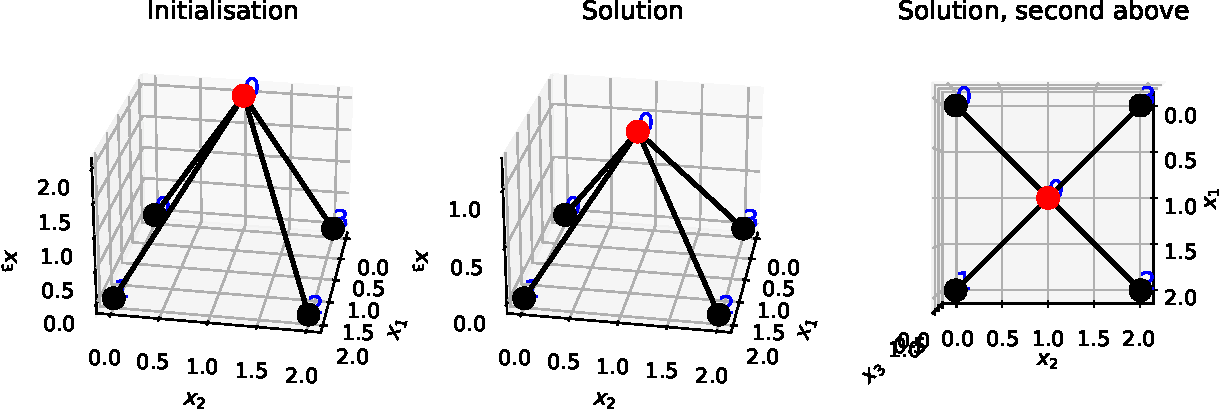
\includegraphics[width=\linewidth]{Bilder/localminpos.pdf}
  \label{fig:}
\end{subfigure}%
\begin{subfigure}{.5\textwidth}
  \centering
  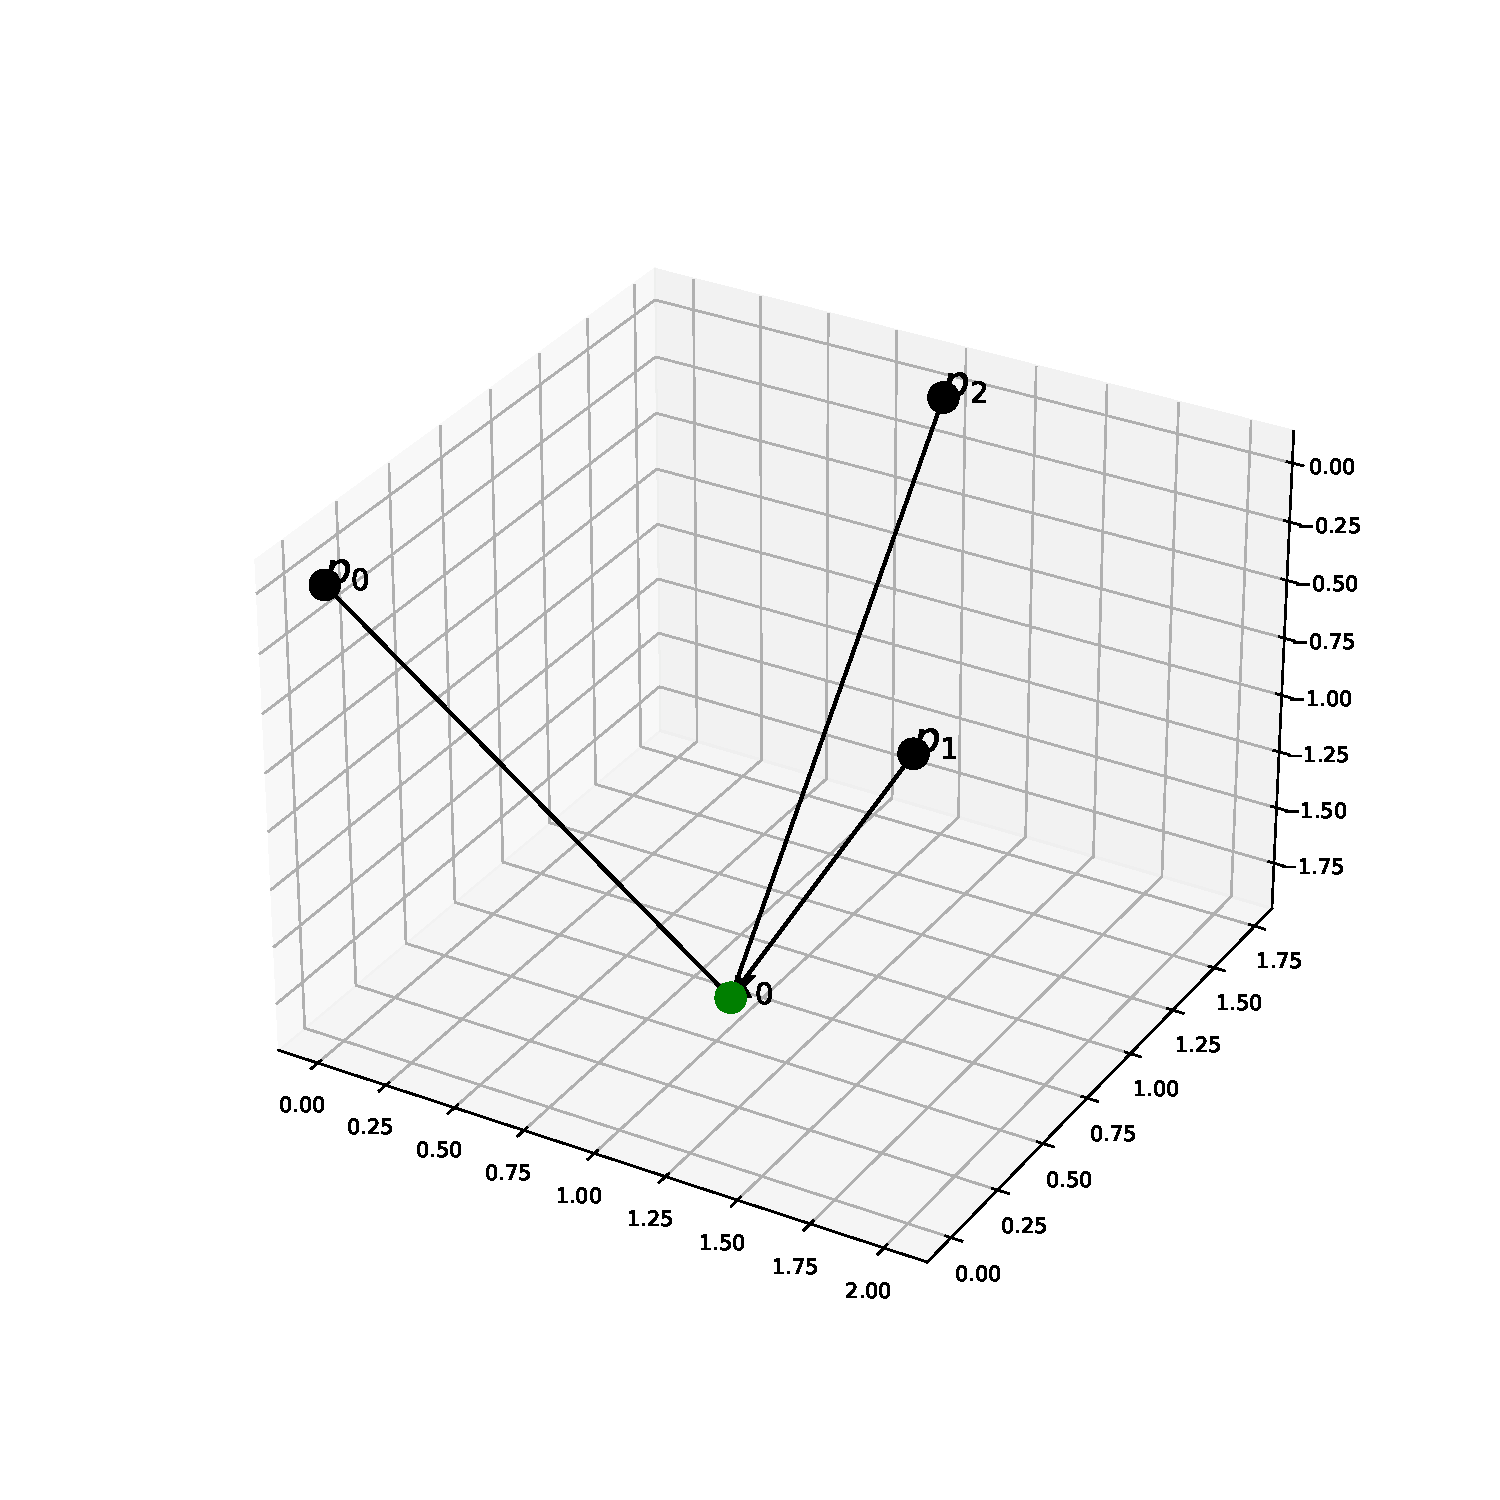
\includegraphics[width=1\linewidth]{Bilder/localminneg.pdf}
  \label{fig:sub2}
\end{subfigure}
\caption{Local optimizer to the left, global optimizer to the right. The free node $x^{(0)}$ is connected through bars to three fixed nodes  $p^{(0)}$, $p^{(1)}$, and $p^{(2)}$.}
\label{fig:local_optimizer}
\end{figure}

Fix a three nodes $p^{(0)}$, $p^{(1)}$, and $p^{(2)}$, and consider a free node $x^{(0)}$ that initially is placed above the $xy$-plane. The position of $x^{(0)}$ will be determined by  
At this starting position the bar will not have any elastic energy, so the gravity will bring the node downwards until the gravity is equally strong as the elastic force from the bar, which will be a local minima. However, it will not be a global minima as we will have lower energy if we instead placed $x^{(2)}$ below $p^{(1)}$ as seen in the rightmost illustration. 



\section{Tensegrity domes in constrained optimization}\label{sec:freestanding}
We will now consider the full problem \eqref{energy} with the constraints given by 
\begin{equation}
    x_3^{(i)} \geq 0 \quad \forall \quad i = 1,...,N \label{eq:aboveground}
\end{equation}

As this is a constrained optimization problem, we define the Lagrangian \begin{equation}
    \mathcal{L}(X,\lambda) = E(X) - \sum_{i \in \ \mathcal{I}}\lambda_i c_i(X)
\end{equation}
Where $c_i(X) = x^{(i)}_3$.

The first order optimality conditions for a given $(X^*,\lambda^*)$ are \begin{equation}
\begin{aligned}
       &\nabla_x \mathcal{L}(X,\lambda^*)=0\\ 
       &x^{*(i)}_3 \geq 0,\quad i = 1,...,N\\
       &\lambda_i^* \geq 0 ,\quad i = 1,...,N\\
       & \lambda_i^* x^{*(i)}_3 = 0,\quad i = 1,...,N
\end{aligned}
\end{equation}
As for LICQ we have 

\begin{align*}
    \nabla c_1(X) = \bigg( \frac{\partial c_1}{\partial x^{(1)}},\frac{\partial c_1}{\partial x^{(2)}},...,\frac{\partial c_1}{\partial x^{(i)}},...,\frac{\partial c_1}{\partial x^{(N)}} \bigg) =\bigg( (0,0,1),(0,0,0),...,(0,0,0),...,(0,0,0) \bigg) \\
    \nabla c_2(X) = \bigg( (0,0,0),(0,0,1),...,(0,0,0),...,(0,0,0) \bigg) \\
    \vdots 
    \hspace{200pt}\\
    \nabla c_i(X) = \bigg( (0,0,0),(0,0,0),...,\underbrace{(0,0,1)}_{i^{\text{th}}\text{ term}},...,(0,0,0) \bigg)\\
    \vdots
    \hspace{200pt}\\
    \nabla c_N(X) = \bigg( (0,0,0),(0,0,0),...,(0,0,0),...,(0,0,1) \bigg) \\
\end{align*}

It's clear that the inequality constraints $\{\nabla c_i(X),i=1,2,...,N\}$ are linearly independent as there are no vectors with non-zero terms in the same dimension. This means LICQ holds, and therefore the KKT conditions are neccesary, but they are not sufficient as our problem is not convex.